\section{Identified Challenges and Project Concept}
DDI is potentially a very useful digital artefact - a DDI is a versatile dependability assurance case, the utility of which spans from component design to in-the-field operation of a CPS. However, the production and use of DDIs for heterogeneous systems poses a number of significant technological and engineering challenges that are pertinent and important in industry and motivate the objectives of the DEIS project. 

The DEIS project identifies the following challenges for the use of DDI:

\begin{enumerate}
	\item \textbf{Universal exchange of dependability information}
		\begin{itemize}
			\item Currently there is a lack of common model representations for the exchange of dependability information. Thus, a precondition for DDI is the existence of an open dependability metamodel. 
			\item DDIs should be sufficiently expressive to enable the component integrator to compile DDIs from the sub-components DDIs, for system synthesis.
			\item DDIs should optionally shield sensitive details through abstraction to protect the component provider's intellectual property. 
		\end{itemize}
	\item \textbf{Efficient dependability assurance across industries and value chains}
		\begin{itemize}
			\item Component provider should be able to generate DDIs based on the dependability information of their components/systems that is already available in their existing tools.
			\item It must be possible to include the information contained in DDIs into the dependability assurance lifecycle and tool chain of the component integrator, to cater with the change in component/system requirements and integration context.
			\item Dependability should be considered from the early stages of design, so that a model-based approach can be adopted to enable automation, and eventually the automatic synthesis of systems.
		\end{itemize}
	\item \textbf{Dependable integration of systems in the field}
		\begin{itemize}
			\item In CPS, dependability cannot be fully assured prior to deployment. This requires certain degree of automation in evaluation of DDIs. Thus, DDIs must become executable specifications.
			\item DDIs must be made publicly available to synchronise changes in them.
			\item Fully automated evaluation of DDIs required for highly dynamic environments.
		\end{itemize}
\end{enumerate}

\begin{figure}[ht!]
	\centering
	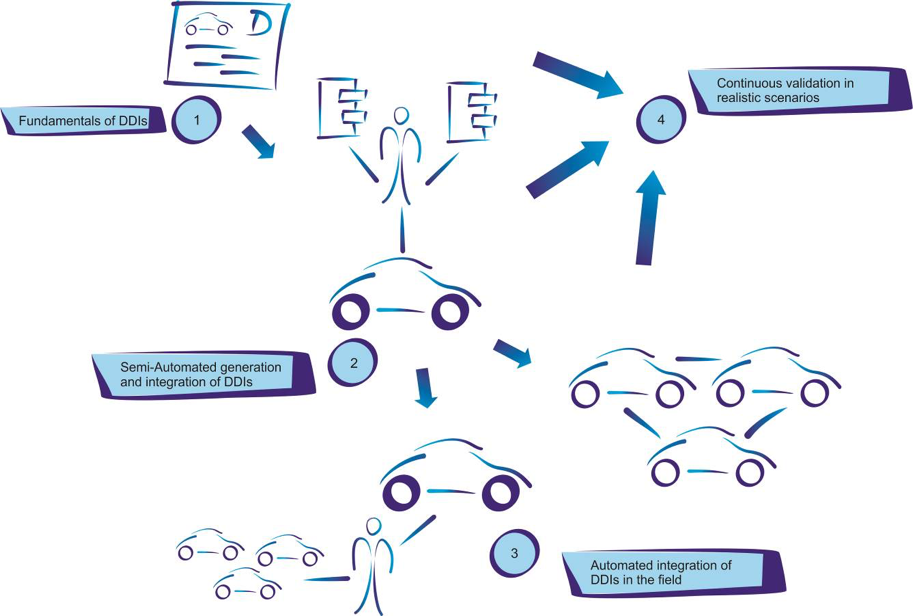
\includegraphics[width=1\linewidth]{./fig/proj_concept.png}
	\caption{DEIS project concept}
	\label{fig:proj_concept}
\end{figure}

To address these major technology and research challenges, the DEIS project sets out a four-stage concept, as illustrated in Figure \ref{fig:proj_concept}. The first stage aims at the fundamentals of DDIs, such as the definition of a universal format of DDIs based on an open information model for the exchange of dependability related information. The second stage is to provide semi-automated and increasingly automated support for generating DDIs out of existing design and safety models as well as for integrating the DDIs of sub-components into DDIs of larger systems by integrators. The third stage facilitates dependable integration of systems in the field though automated evaluation of DDIs that includes the concept of executable DDIs on board. Finally, the fourth stage of the project is to have continuous validation of the project results in realistic scenarios and case studies.



